\section{\textbf{Experimental Setup}}

Implemented in Python, the algorithms feature a graphical user interface (GUI) tailored for interactive visualization.
This GUI facilitates user engagement by enabling the input of points or line segments, the selection of a specific
algorithm, and the observation of the corresponding convex hull construction or intersection detection, depending on
the context.


\textbf{Experimental Setup Flow:}
\subsection{}
\textbf{Initialization:}

Set up the Python environment.
Import necessary libraries: tkinter for GUI, matplotlib for plotting, compare to key for sorting, time for measuring execution time, sys for memory usage, and sympy for algebraic computations. Graphical User Interface (GUI) Initialization:

\textbf{For Convex Hull Algorithms:}

Create a GUI for visualizing convex hull construction. Define a canvas for plotting points and convex hulls. Add buttons for each convex hull algorithm (Graham Scan, Jarvis March, Quick Elimination, Andrew's Algorithm, Brute Force). Include buttons for clearing points and displaying time and space complexities.
Design labels for time and space complexities.

\textbf{For Line Segment Intersection Algorithm:} 

Create a GUI for visualizing line segment intersections.
Define a canvas for plotting line segments and intersection points. Add buttons for different line segment intersection methods(Algebraic, CCW Computation, Vector Cross Product).Include buttons for adding points, clearing canvas, and displaying intersection results. Design labels for displaying intersection results.

\subsection{}
\textbf{Algorithm Implementation:}

Implement Convex Hull Algorithms in separate functions/classes.
Graham Scan, Jarvis March, Quick Elimination, Andrew's Algorithm, Brute Force. Implement Line Segment Intersection Algorithm in a separate class. Methods for Algebraic, CCW Computation, Vector Cross Product.

\subsection{}
\textbf{Experimental Execution:}

\textbf{For Convex Hull Algorithms:}

Measure the execution time using the time library.
Measure space complexity using sys.getsizeof().
Update the GUI labels with time and space complexity results.

\textbf{For Line Segment Intersection Algorithm:}

Implement methods to check intersection using different techniques.
Update the GUI labels with intersection results.

\section{\textbf{Results and Discussions:}}

\begin{figure}
    \centering
    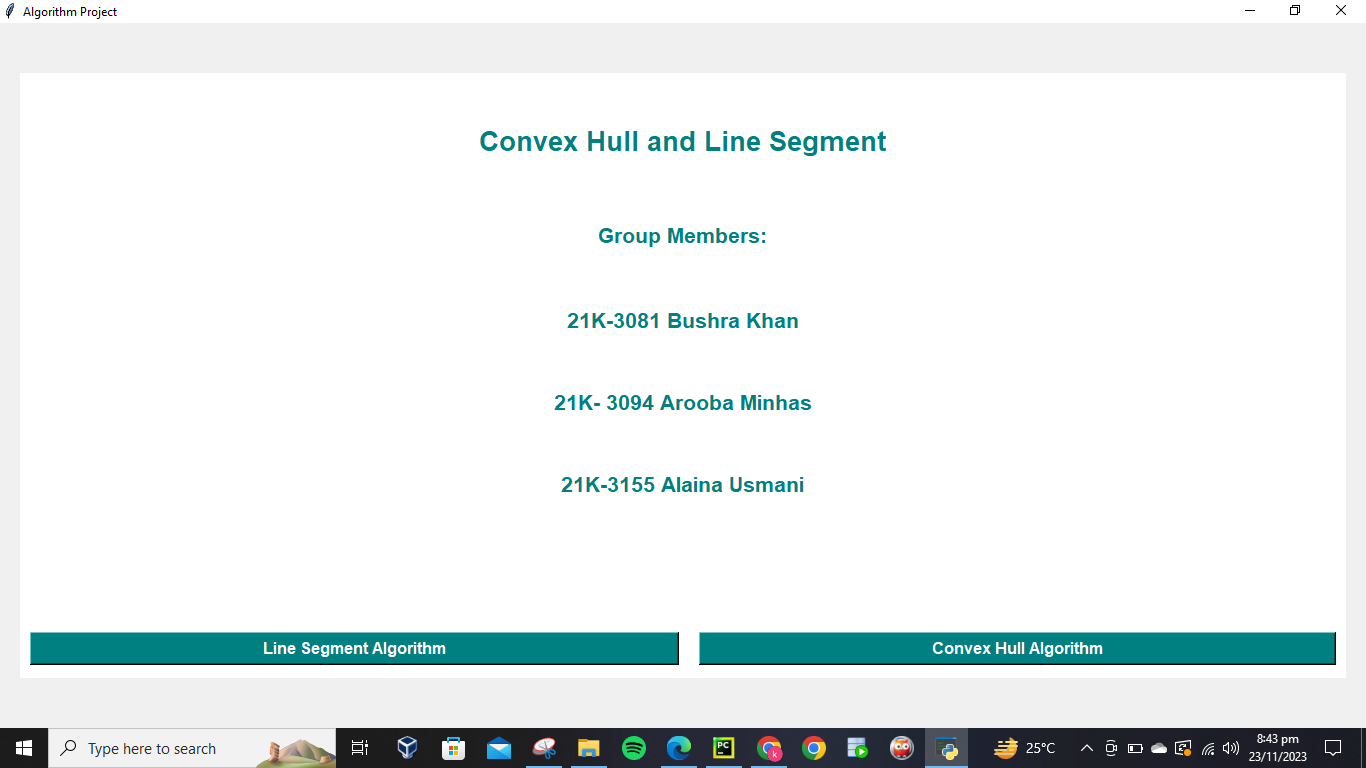
\includegraphics[width=1\linewidth]{p1.PNG}
    \caption{Title Page}
    \label{fig:enter-label}
\end{figure}

\begin{figure}
    \centering
    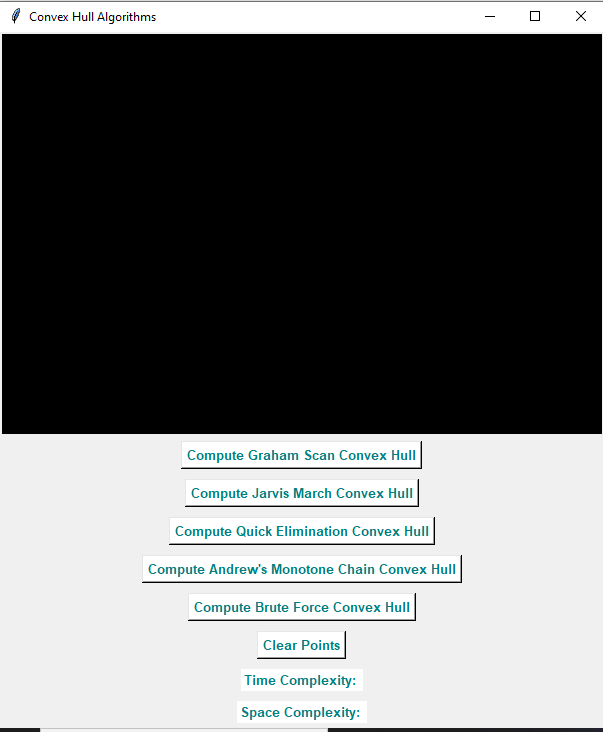
\includegraphics[width=1\linewidth]{p2.PNG}
    \caption{Convex Hull Algorithm Page}
    \label{fig:enter-label}
\end{figure}

\begin{figure}
    \centering
    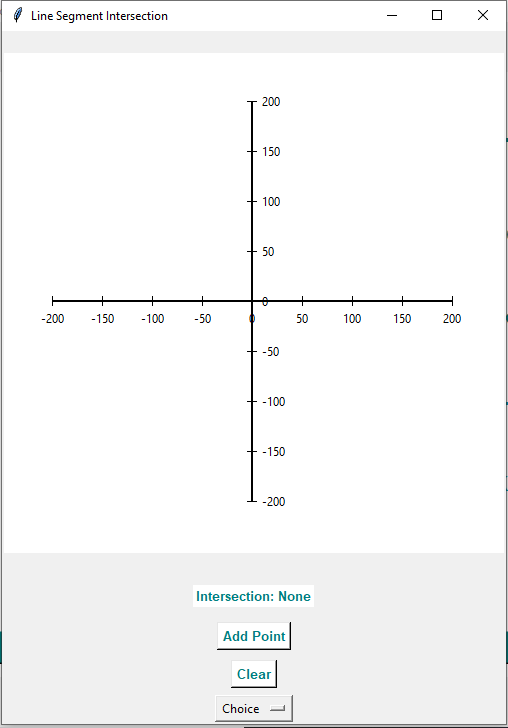
\includegraphics[width=1\linewidth]{p3.PNG}
    \caption{Line Segment Algorithm Page}
    \label{fig:enter-label}
\end{figure}

